Due to the higher computational cost of computing frequentist confidence intervals by generating pseudodata to estimate the test-statistic ($\mathcal{TS}$) distribution, it is common to use the approximation given by Wilks' theorem for the cases where the underlying hypotheses hold. In the case of small MC, a likelihood description that neglects MC uncertainties may lead to undercoverage even for a large data sample. In this section, we will use  $\mathcal{TS}=\Delta l=l(\vectheta_{\rm true})-l(\hat{\vectheta})$, where $\vectheta_{\rm true}$ and $\hat{\vectheta}$ correspond to the true and best-fit $(\Omega, \Phi)$, respectively. We evaluate the coverage properties, computed using the asymptotic approximation given by Wilks' theorem, of the two-dimensional fit over $(\Omega, \Phi)$ for several likelihood constructions. These include the modified-$\chi^2$, $\adhoc$, $\lbarlow$, $\meanl$, and $\mcl$. These five test-statistics were chosen on the basis of their computation speed and as tests of different approaches towards the treatment of weighted MC. Note that using Wilks' theorem is an approximation and in general we encourage the reader to perform coverage tests for their own particular setup.

\begin{figure}[htp]
\centering
\centering
    \subfloat{
        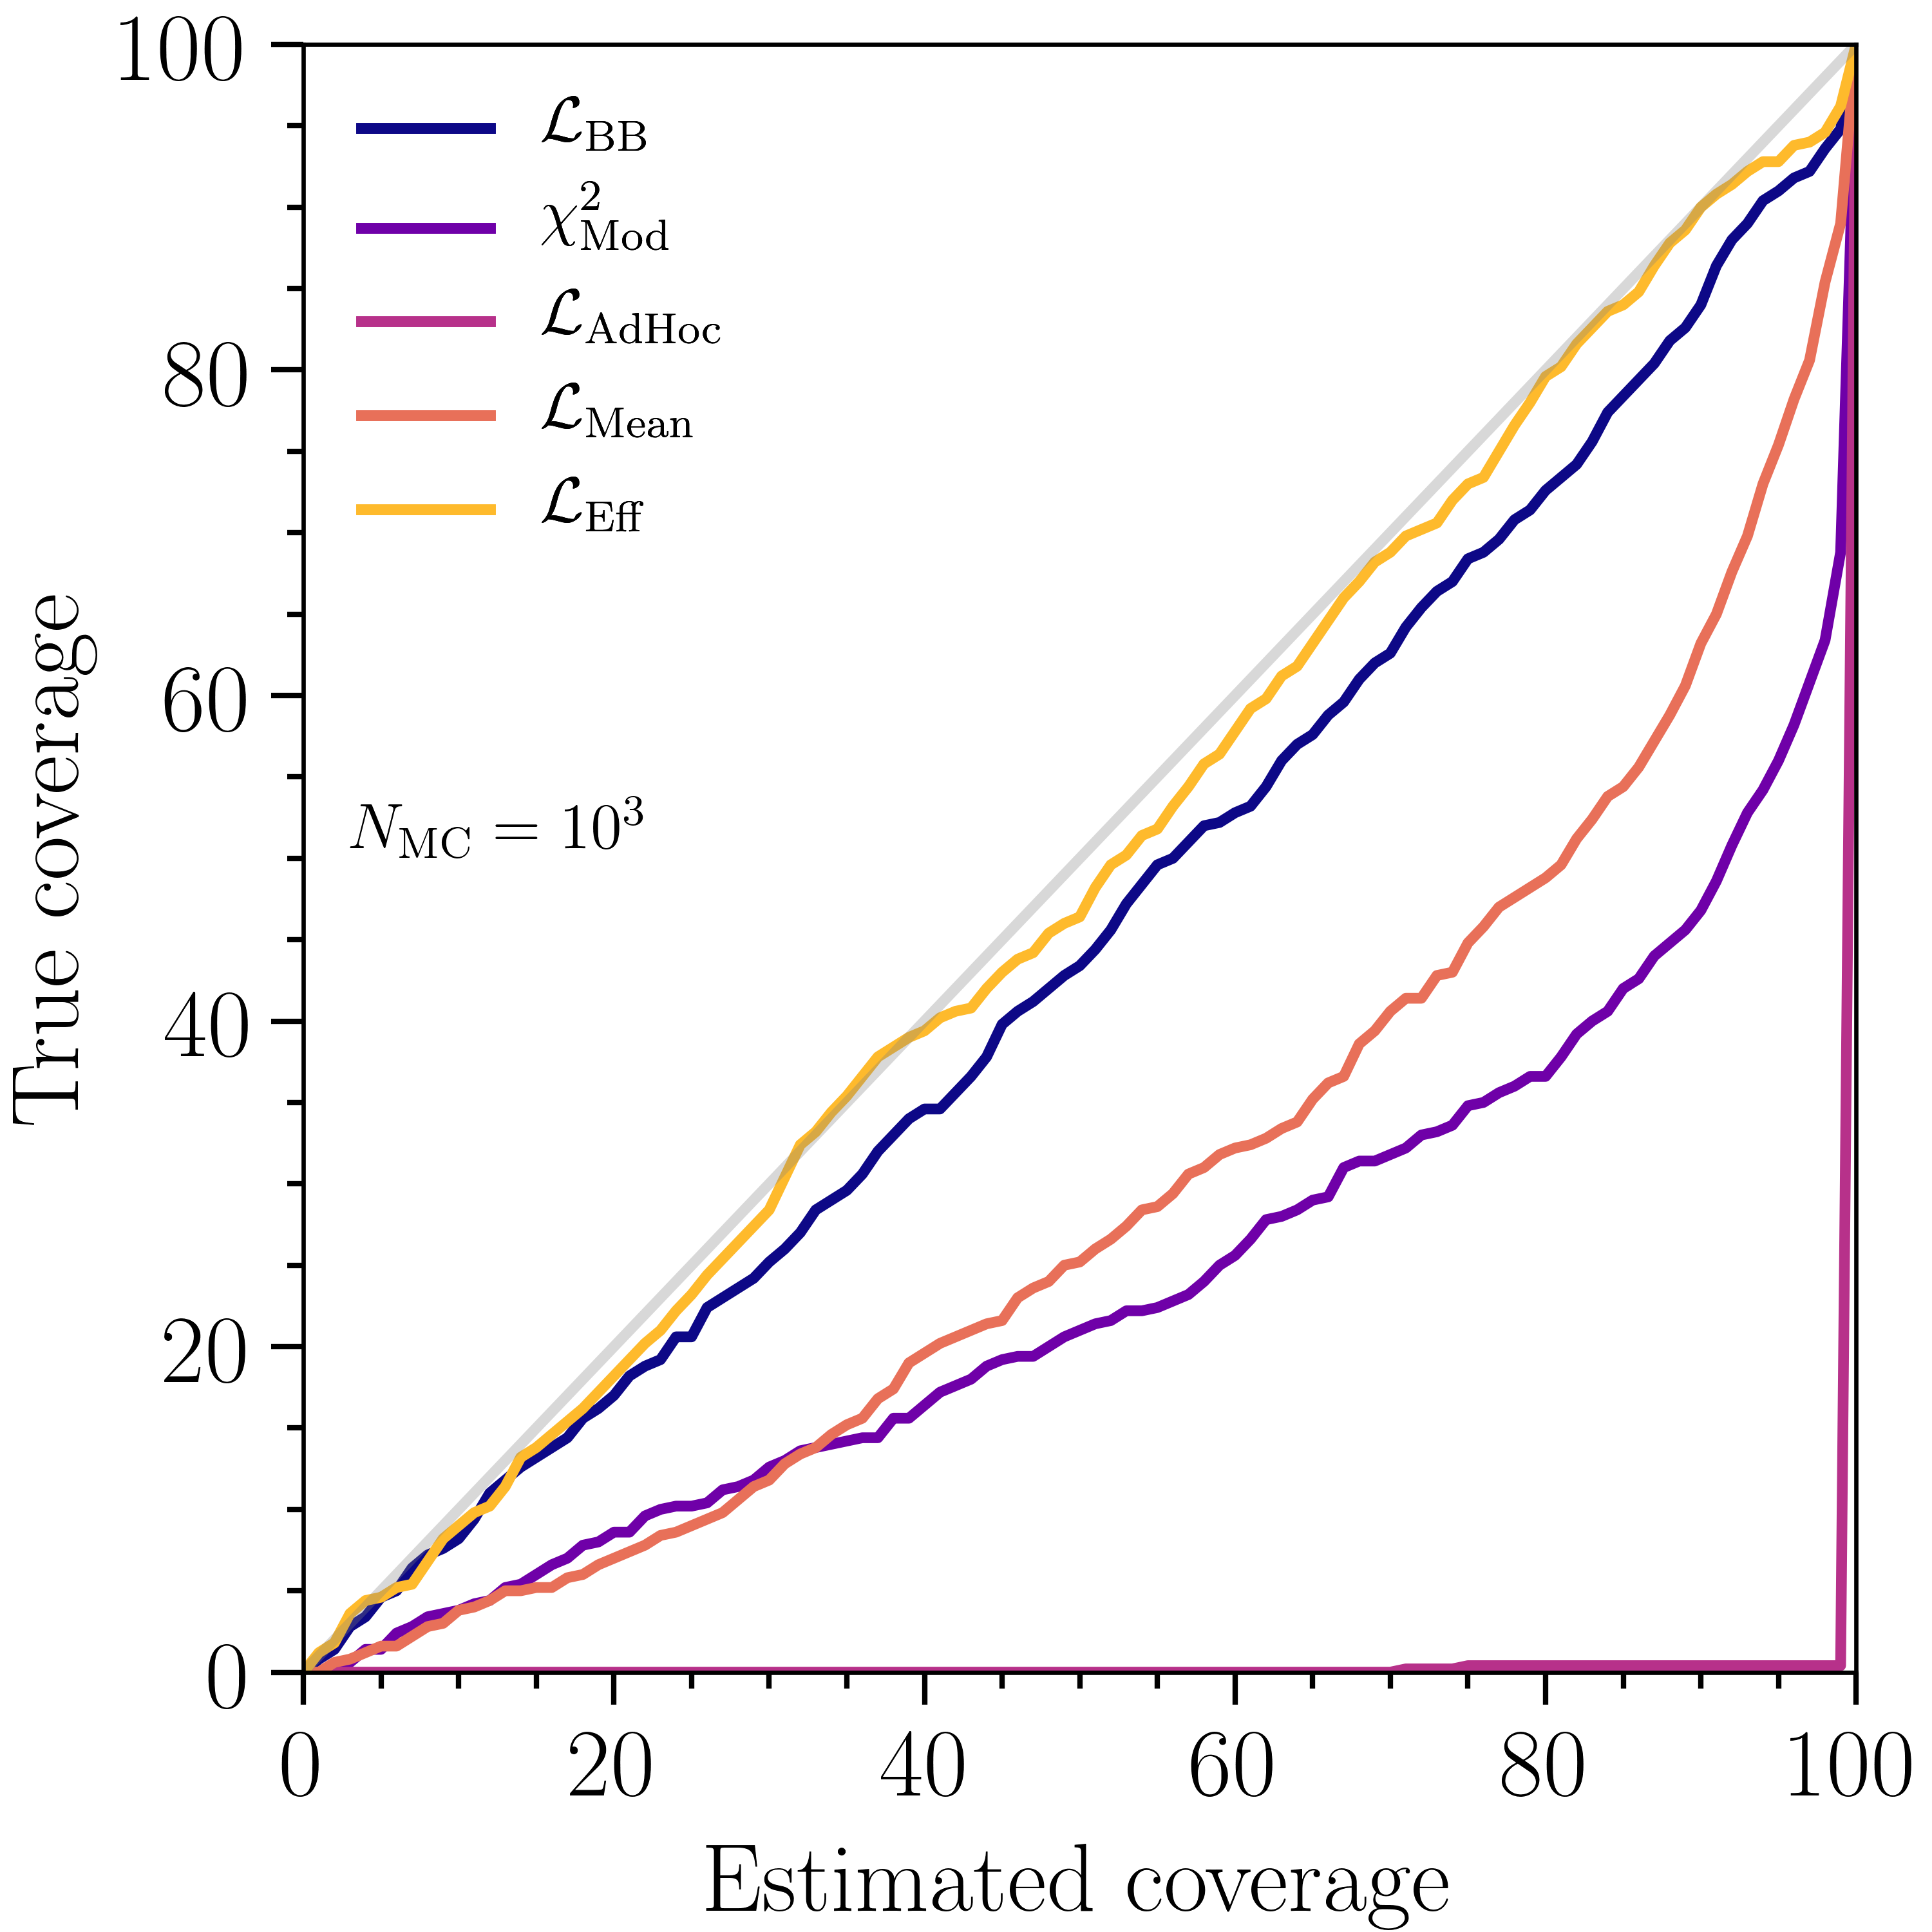
\includegraphics[width=0.48\linewidth]{{{fig/fig5_1_1e3}}}
    }
    \subfloat{
        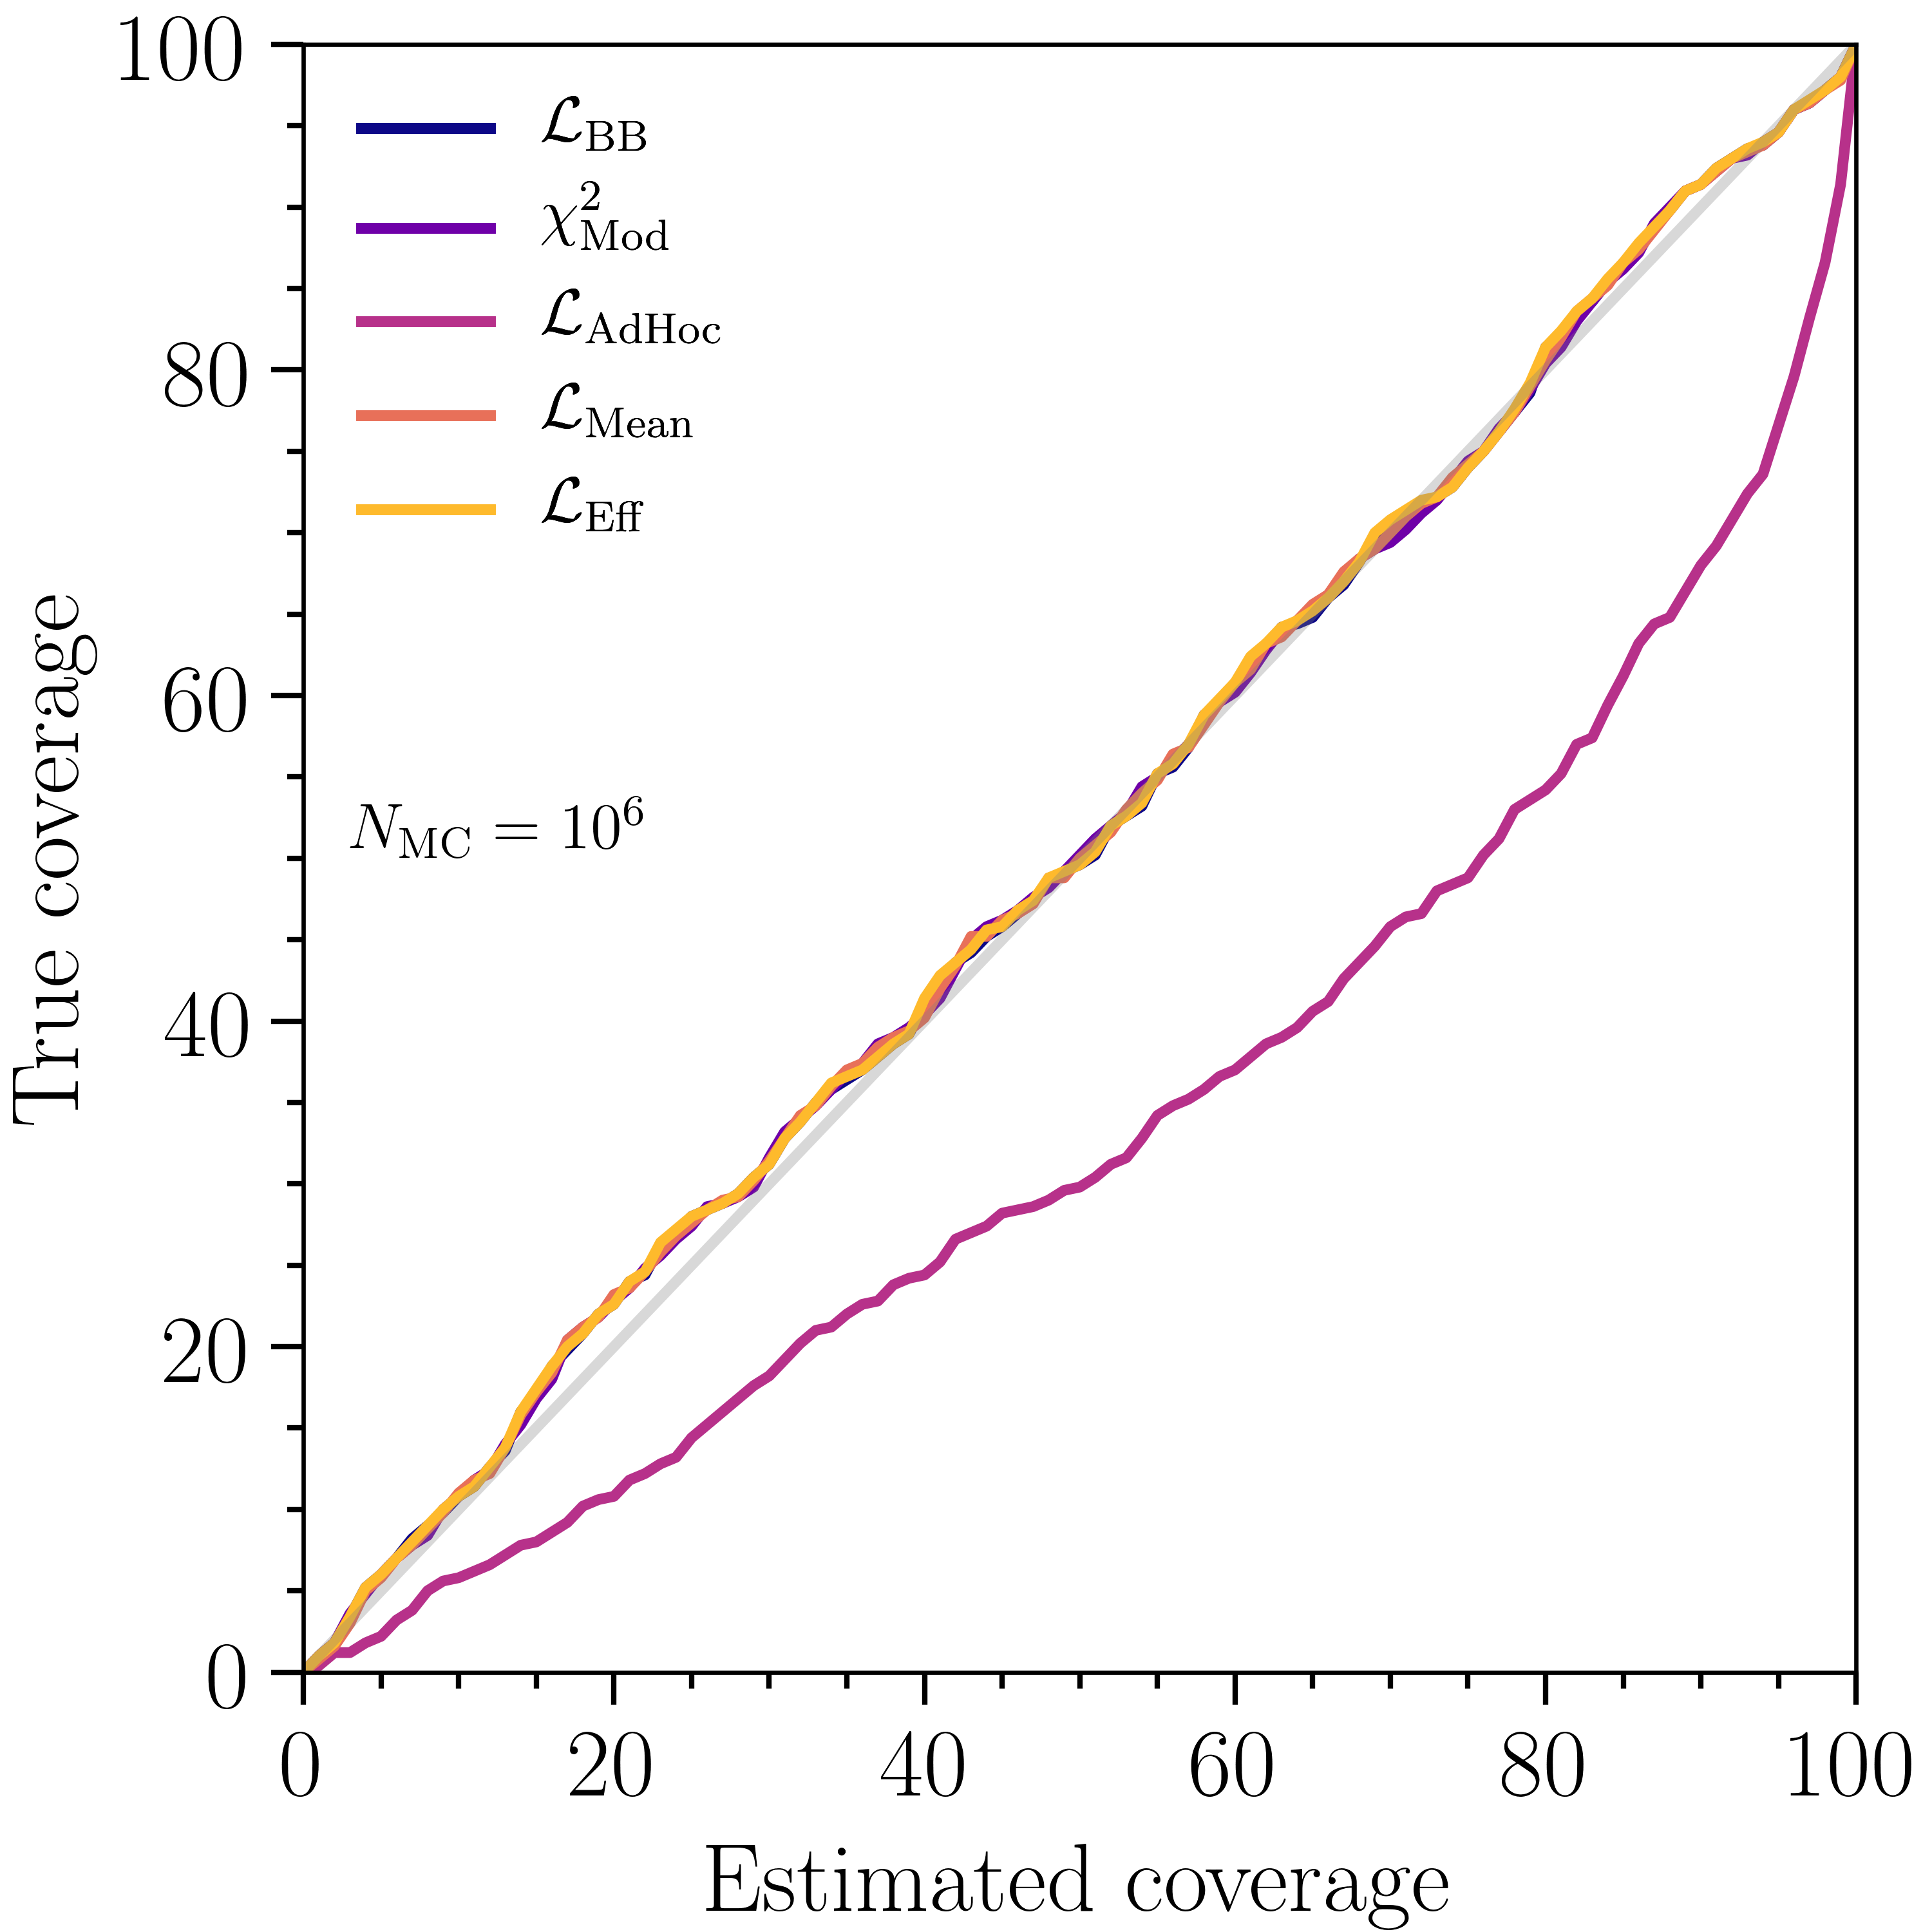
\includegraphics[width=0.48\linewidth]{fig/fig5_1_1e6}
    }
\caption{\textbf{\textit{Coverage properties.}} True coverage of the Wilks' confidence interval for two sets of toy experiments with different MC sizes: $10^3$ events (left) and $10^6$ events (right). The ad hoc Poisson likelihood severely undercovers. The modified-$\chi^2$, $\lbarlow$, and $\meanl$ also undercover for small MC size. The effective likelihood, $\mcl$, derived in Sec.~\ref{sec:constructing} performs best.}
\label{fig:coverage}
\end{figure}

Several configurations were tested, all under the assumptions of the toy experiment described in Sec.~\ref{sec:pointestimation}. The MC was generated for two different settings of the total number of events: $10^3$ and $10^6$. For each setting, 500 toy experiments were generated, their best-fits found, and their $\Delta l$ evaluated. Each toy experiment was classified as covering $\vectheta_{\rm true}$ at a specified level $p$ if $\Delta l < I(p;2)$, where $I$ is the inverse of the $\chi^2$ cumulative density function and $2$ indicates the number of degrees of freedom.

Figure~\ref{fig:coverage} shows the percentage of times the true parameters were within the confidence intervals at level $p$ as a function of the estimated coverage percentile for that level. First note that, as expected, the true coverage is highly dependent on MC size, with higher MC size leading towards improved agreement. In the case of $N_\mathrm{MC}=10^3$, $\lbarlow$, $\meanl$, modified-$\chi^2$, and $\adhoc$ all undercover to varying degrees of severeness. For $N_\mathrm{MC}=10^6$, $\adhoc$ still undercovers, which is not surprising as it presumes zero MC uncertainty, but the other likelihoods exhibit good agreement. In this benchmark test, $\mcl$ exhibits the best coverage properties. However, note that using Wilks’ theorem in order to evaluate confidence intervals implies an asymptotic approximation. In general, this approximation does not necessarily have to hold and we encourage the reader to always perform their own coverage tests suitable for their particular experimental setup.
